\documentclass[tikz,border=2pt]{standalone}
\usepackage{pgfplots}
\pgfplotsset{compat=1.18}
\definecolor{raisedgreen}{HTML}{1A7F37}
\definecolor{regressionred}{HTML}{CF222E}
\begin{document}
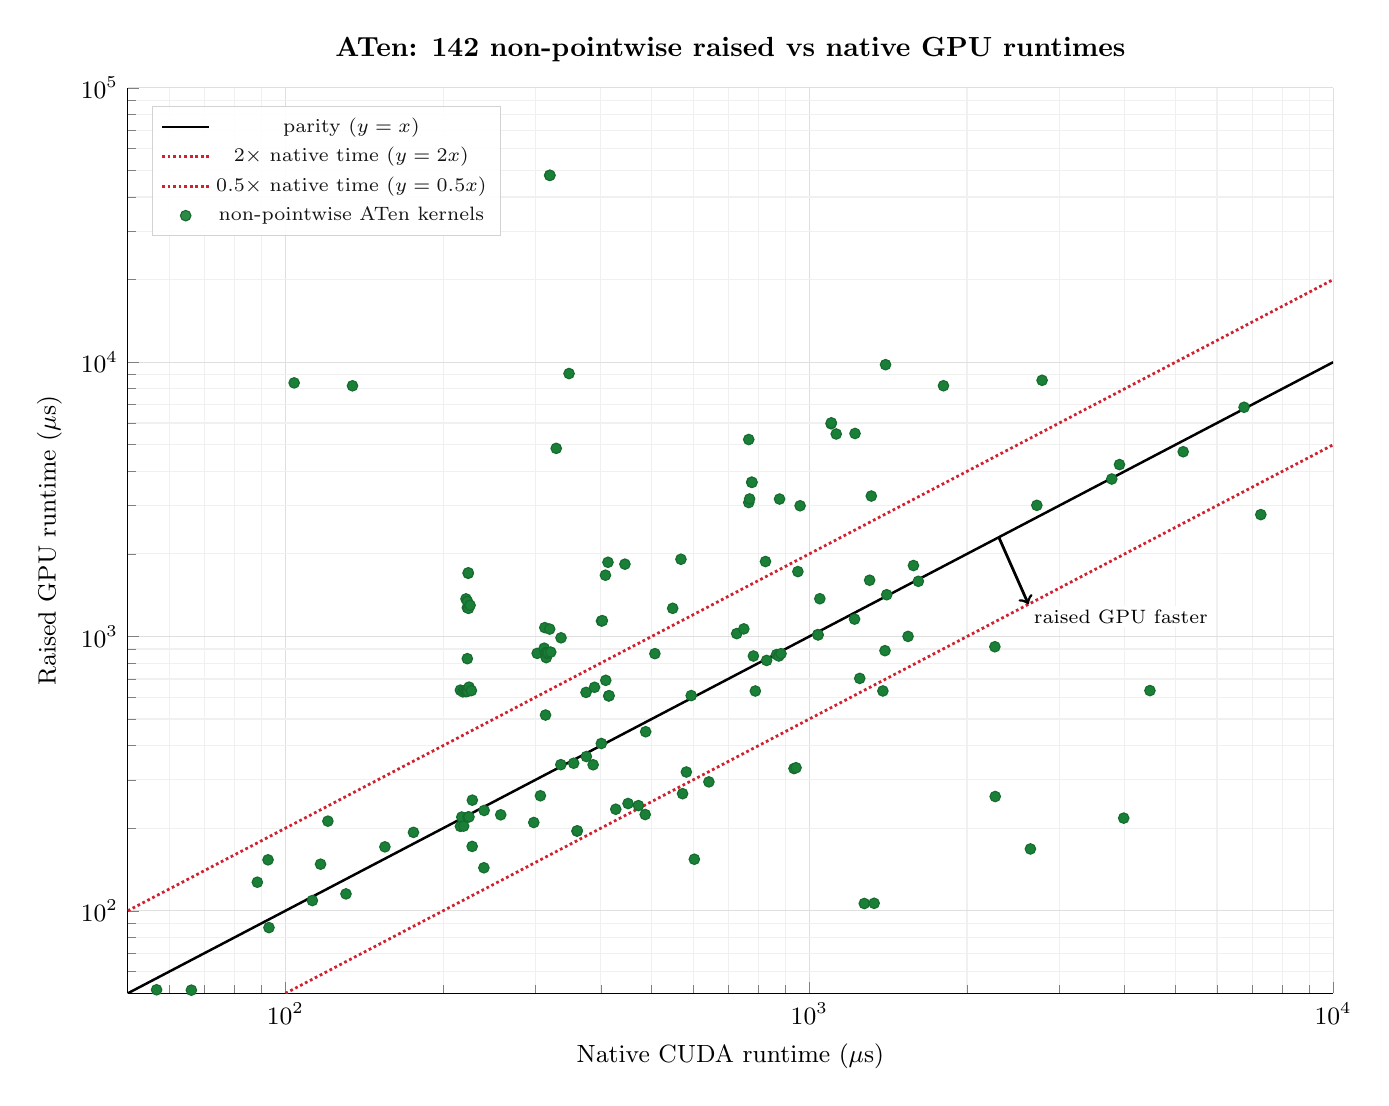
\begin{tikzpicture}
\begin{loglogaxis}[
  width=6.65in, height=5.15in,
  title={ATen: 142 non-pointwise raised vs native GPU runtimes},
  title style={font=\bfseries\normalsize},
  xlabel={Native CUDA runtime ($\mu$s)},
  ylabel={Raised GPU runtime ($\mu$s)},
  xmin=50, xmax=10000, ymin=50, ymax=100000,
  grid=both, minor grid style={draw=gray!12},
  major grid style={draw=gray!25},
  ticklabel style={font=\small}, label style={font=\small},
  legend style={font=\scriptsize,at={(0.02,0.98)},anchor=north west,
                 fill=white,fill opacity=0.92,draw=gray!35},
  axis lines*=left,
]
\addplot+[no marks,draw=black,line width=0.9pt]
  coordinates {(50,50) (10000,10000)};
\addlegendentry{parity ($y=x$)}
\addplot+[no marks,draw=regressionred,densely dotted,line width=1.0pt]
  coordinates {(50,100) (10000,20000)};
\addlegendentry{$2\times$ native time ($y=2x$)}
\addplot+[no marks,draw=regressionred,densely dotted,line width=1.0pt]
  coordinates {(100,50) (10000,5000)};
\addlegendentry{$0.5\times$ native time ($y=0.5x$)}
\addplot+[only marks,mark=*,mark size=1.9pt,
  draw=raisedgreen!85!black,fill=raisedgreen]
  coordinates {(22.816000,49.087997) (56.768000,51.520020) (66.144000,51.360352) (88.384000,127.104004) (92.640000,153.375977) (93.024000,86.815994) (103.904000,8403.584000) (112.576000,108.959961) (116.704000,147.872000) (120.512000,212.224121) (130.496000,115.231995) (134.272000,8199.967773) (154.848000,171.040009) (175.552000,193.152008) (215.744000,637.408005) (215.808000,203.104004) (217.088000,219.616013) (218.176000,628.255997) (218.880000,203.584000) (219.680000,635.679993) (221.120000,629.248001) (221.152000,1370.912003) (222.144000,635.552002) (222.432000,830.080002) (222.464000,1273.824005) (222.592000,1342.431992) (222.880000,631.039993) (223.136000,219.743988) (223.296000,1699.552002) (223.360000,1706.783997) (223.648000,1266.176010) (224.064000,219.903992) (224.160000,653.728012) (225.152000,1299.807999) (226.464000,635.007996) (227.232000,171.647995) (227.392000,253.088013) (239.232000,143.487999) (239.520000,232.095993) (257.632000,223.807999) (297.920000,209.824001) (302.368000,867.776001) (306.688000,262.591797) (311.840000,906.335999) (312.704000,1077.215988) (313.696000,517.087997) (313.728000,869.919998) (314.048000,873.184006) (314.176000,871.936005) (314.592000,839.680000) (314.688000,837.471998) (315.872000,865.983994) (317.376000,872.127991) (319.456000,1064.063995) (319.488000,47972.896000) (319.840000,47992.480000) (320.992000,877.087997) (328.800000,4850.496094) (335.520000,340.959991) (335.808000,988.671875) (347.872000,9089.823999) (355.008000,345.087997) (360.192000,195.200001) (360.704000,195.648001) (374.848000,625.472000) (375.392000,365.023987) (386.688000,340.640137) (389.120000,652.800003) (400.896000,407.264008) (401.152000,1138.528000) (402.720000,1142.079987) (408.160000,1672.672012) (408.768000,692.063965) (412.768000,1864.224001) (414.080000,607.007999) (414.848000,608.416000) (427.136000,234.528000) (444.672000,1835.007812) (450.816000,246.048004) (471.968000,241.759995) (486.144000,224.352005) (487.104000,449.503906) (507.264000,865.855988) (548.512000,1266.592010) (568.832000,1912.447998) (572.896000,267.232010) (582.528000,320.575989) (595.072000,608.832001) (603.328000,154.144043) (643.200000,295.040009) (726.848000,1024.416000) (749.984000,1065.632000) (766.368000,3078.559998) (766.464000,5224.896000) (769.216000,3172.031738) (776.160000,3650.368164) (777.536000,3647.808105) (782.208000,848.640001) (788.928000,632.736008) (824.768000,1876.448000) (828.896000,817.856001) (866.080000,859.007996) (874.880000,848.896000) (877.408000,3169.823730) (883.040000,865.695999) (934.976000,329.983999) (943.200000,332.288000) (950.976000,1724.255997) (960.320000,2995.936035) (1038.080000,1016.000000) (1039.584000,1013.024000) (1047.328000,1372.671997) (1100.352000,5961.791992) (1101.760000,6008.960007) (1125.600000,5472.800003) (1220.096000,1156.832031) (1222.496000,5495.456009) (1248.096000,703.360352) (1273.248000,106.304001) (1303.488000,1603.680176) (1313.152000,3251.135742) (1329.600000,106.495605) (1381.760000,633.024002) (1394.624000,887.520020) (1398.112000,9793.119995) (1405.312000,1419.679993) (1543.424000,1000.671875) (1580.576000,1814.399994) (1614.784000,1588.832001) (1803.584000,8205.024002) (2260.544000,917.407999) (2263.808000,260.959961) (2642.624000,168.032000) (2718.496000,3006.496002) (2781.824000,8587.552246) (3778.624000,3750.080002) (3909.408000,4233.151855) (3982.368000,217.664001) (4468.640000,634.975998) (5172.288000,4714.207993) (6758.560000,6848.479996) (7274.784000,2781.216000)};
\addlegendentry{non-pointwise ATen kernels}
\draw[->,black,line width=1.0pt]
  (axis cs:2300,2300) -- (axis cs:2620,1310)
  node[pos=1,below right,font=\scriptsize,fill=white,inner sep=1.5pt]
  {raised GPU faster};
\end{loglogaxis}
\end{tikzpicture}
\end{document}
